
%% bare_jrnl.tex
%% V1.3
%% 2007/01/11
%% by Michael Shell
%% see http://www.michaelshell.org/
%% for current contact information.
%%
%% This is a skeleton file demonstrating the use of IEEEtran.cls
%% (requires IEEEtran.cls version 1.7 or later) with an IEEE journal paper.
%%
%% Support sites:
%% http://www.michaelshell.org/tex/ieeetran/
%% http://www.ctan.org/tex-archive/macros/latex/contrib/IEEEtran/
%% and
%% http://www.ieee.org/



% *** Authors should verify (and, if needed, correct) their LaTeX system  ***
% *** with the testflow diagnostic prior to trusting their LaTeX platform ***
% *** with production work. IEEE's font choices can trigger bugs that do  ***
% *** not appear when using other class files.                            ***
% The testflow support page is at:
% http://www.michaelshell.org/tex/testflow/


%%*************************************************************************
%% Legal Notice:
%% This code is offered as-is without any warranty either expressed or
%% implied; without even the implied warranty of MERCHANTABILITY or
%% FITNESS FOR A PARTICULAR PURPOSE! 
%% User assumes all risk.
%% In no event shall IEEE or any contributor to this code be liable for
%% any damages or losses, including, but not limited to, incidental,
%% consequential, or any other damages, resulting from the use or misuse
%% of any information contained here.
%%
%% All comments are the opinions of their respective authors and are not
%% necessarily endorsed by the IEEE.
%%
%% This work is distributed under the LaTeX Project Public License (LPPL)
%% ( http://www.latex-project.org/ ) version 1.3, and may be freely used,
%% distributed and modified. A copy of the LPPL, version 1.3, is included
%% in the base LaTeX documentation of all distributions of LaTeX released
%% 2003/12/01 or later.
%% Retain all contribution notices and credits.
%% ** Modified files should be clearly indicated as such, including  **
%% ** renaming them and changing author support contact information. **
%%
%% File list of work: IEEEtran.cls, IEEEtran_HOWTO.pdf, bare_adv.tex,
%%                    bare_conf.tex, bare_jrnl.tex, bare_jrnl_compsoc.tex
%%*************************************************************************

% Note that the a4paper option is mainly intended so that authors in
% countries using A4 can easily print to A4 and see how their papers will
% look in print - the typesetting of the document will not typically be
% affected with changes in paper size (but the bottom and side margins will).
% Use the testflow package mentioned above to verify correct handling of
% both paper sizes by the user's LaTeX system.
%
% Also note that the "draftcls" or "draftclsnofoot", not "draft", option
% should be used if it is desired that the figures are to be displayed in
% draft mode.
%
\documentclass[journal]{IEEEtran}
%
% If IEEEtran.cls has not been installed into the LaTeX system files,
% manually specify the path to it like:
% \documentclass[journal]{../sty/IEEEtran}





% Some very useful LaTeX packages include:
% (uncomment the ones you want to load)


% *** MISC UTILITY PACKAGES ***
%
%\usepackage{ifpdf}
% Heiko Oberdiek's ifpdf.sty is very useful if you need conditional
% compilation based on whether the output is pdf or dvi.
% usage:
% \ifpdf
%   % pdf code
% \else
%   % dvi code
% \fi
% The latest version of ifpdf.sty can be obtained from:
% http://www.ctan.org/tex-archive/macros/latex/contrib/oberdiek/
% Also, note that IEEEtran.cls V1.7 and later provides a builtin
% \ifCLASSINFOpdf conditional that works the same way.
% When switching from latex to pdflatex and vice-versa, the compiler may
% have to be run twice to clear warning/error messages.






% *** CITATION PACKAGES ***
%
\usepackage{cite}
% cite.sty was written by Donald Arseneau
% V1.6 and later of IEEEtran pre-defines the format of the cite.sty package
% \cite{} output to follow that of IEEE. Loading the cite package will
% result in citation numbers being automatically sorted and properly
% "compressed/ranged". e.g., [1], [9], [2], [7], [5], [6] without using
% cite.sty will become [1], [2], [5]--[7], [9] using cite.sty. cite.sty's
% \cite will automatically add leading space, if needed. Use cite.sty's
% noadjust option (cite.sty V3.8 and later) if you want to turn this off.
% cite.sty is already installed on most LaTeX systems. Be sure and use
% version 4.0 (2003-05-27) and later if using hyperref.sty. cite.sty does
% not currently provide for hyperlinked citations.
% The latest version can be obtained at:
% http://www.ctan.org/tex-archive/macros/latex/contrib/cite/
% The documentation is contained in the cite.sty file itself.






% *** GRAPHICS RELATED PACKAGES ***
%
\ifCLASSINFOpdf
  % \usepackage[pdftex]{graphicx}
  % declare the path(s) where your graphic files are
  % \graphicspath{{../pdf/}{../jpeg/}}
  % and their extensions so you won't have to specify these with
  % every instance of \includegraphics
  % \DeclareGraphicsExtensions{.pdf,.jpeg,.png}
\else
  % or other class option (dvipsone, dvipdf, if not using dvips). graphicx
  % will default to the driver specified in the system graphics.cfg if no
  % driver is specified.
  % \usepackage[dvips]{graphicx}
  % declare the path(s) where your graphic files are
  % \graphicspath{{../eps/}}
  % and their extensions so you won't have to specify these with
  % every instance of \includegraphics
  % \DeclareGraphicsExtensions{.eps}
\fi
% graphicx was written by David Carlisle and Sebastian Rahtz. It is
% required if you want graphics, photos, etc. graphicx.sty is already
% installed on most LaTeX systems. The latest version and documentation can
% be obtained at: 
% http://www.ctan.org/tex-archive/macros/latex/required/graphics/
% Another good source of documentation is "Using Imported Graphics in
% LaTeX2e" by Keith Reckdahl which can be found as epslatex.ps or
% epslatex.pdf at: http://www.ctan.org/tex-archive/info/
%
% latex, and pdflatex in dvi mode, support graphics in encapsulated
% postscript (.eps) format. pdflatex in pdf mode supports graphics
% in .pdf, .jpeg, .png and .mps (metapost) formats. Users should ensure
% that all non-photo figures use a vector format (.eps, .pdf, .mps) and
% not a bitmapped formats (.jpeg, .png). IEEE frowns on bitmapped formats
% which can result in "jaggedy"/blurry rendering of lines and letters as
% well as large increases in file sizes.
%
% You can find documentation about the pdfTeX application at:
% http://www.tug.org/applications/pdftex





% *** MATH PACKAGES ***
%
%\usepackage[cmex10]{amsmath}
% A popular package from the American Mathematical Society that provides
% many useful and powerful commands for dealing with mathematics. If using
% it, be sure to load this package with the cmex10 option to ensure that
% only type 1 fonts will utilized at all point sizes. Without this option,
% it is possible that some math symbols, particularly those within
% footnotes, will be rendered in bitmap form which will result in a
% document that can not be IEEE Xplore compliant!
%
% Also, note that the amsmath package sets \interdisplaylinepenalty to 10000
% thus preventing page breaks from occurring within multiline equations. Use:
%\interdisplaylinepenalty=2500
% after loading amsmath to restore such page breaks as IEEEtran.cls normally
% does. amsmath.sty is already installed on most LaTeX systems. The latest
% version and documentation can be obtained at:
% http://www.ctan.org/tex-archive/macros/latex/required/amslatex/math/





% *** SPECIALIZED LIST PACKAGES ***
%
%\usepackage{algorithmic}
% algorithmic.sty was written by Peter Williams and Rogerio Brito.
% This package provides an algorithmic environment fo describing algorithms.
% You can use the algorithmic environment in-text or within a figure
% environment to provide for a floating algorithm. Do NOT use the algorithm
% floating environment provided by algorithm.sty (by the same authors) or
% algorithm2e.sty (by Christophe Fiorio) as IEEE does not use dedicated
% algorithm float types and packages that provide these will not provide
% correct IEEE style captions. The latest version and documentation of
% algorithmic.sty can be obtained at:
% http://www.ctan.org/tex-archive/macros/latex/contrib/algorithms/
% There is also a support site at:
% http://algorithms.berlios.de/index.html
% Also of interest may be the (relatively newer and more customizable)
% algorithmicx.sty package by Szasz Janos:
% http://www.ctan.org/tex-archive/macros/latex/contrib/algorithmicx/




% *** ALIGNMENT PACKAGES ***
%
%\usepackage{array}
% Frank Mittelbach's and David Carlisle's array.sty patches and improves
% the standard LaTeX2e array and tabular environments to provide better
% appearance and additional user controls. As the default LaTeX2e table
% generation code is lacking to the point of almost being broken with
% respect to the quality of the end results, all users are strongly
% advised to use an enhanced (at the very least that provided by array.sty)
% set of table tools. array.sty is already installed on most systems. The
% latest version and documentation can be obtained at:
% http://www.ctan.org/tex-archive/macros/latex/required/tools/


%\usepackage{mdwmath}
%\usepackage{mdwtab}
% Also highly recommended is Mark Wooding's extremely powerful MDW tools,
% especially mdwmath.sty and mdwtab.sty which are used to format equations
% and tables, respectively. The MDWtools set is already installed on most
% LaTeX systems. The lastest version and documentation is available at:
% http://www.ctan.org/tex-archive/macros/latex/contrib/mdwtools/


% IEEEtran contains the IEEEeqnarray family of commands that can be used to
% generate multiline equations as well as matrices, tables, etc., of high
% quality.


%\usepackage{eqparbox}
% Also of notable interest is Scott Pakin's eqparbox package for creating
% (automatically sized) equal width boxes - aka "natural width parboxes".
% Available at:
% http://www.ctan.org/tex-archive/macros/latex/contrib/eqparbox/





% *** SUBFIGURE PACKAGES ***
%\usepackage[tight,footnotesize]{subfigure}
% subfigure.sty was written by Steven Douglas Cochran. This package makes it
% easy to put subfigures in your figures. e.g., "Figure 1a and 1b". For IEEE
% work, it is a good idea to load it with the tight package option to reduce
% the amount of white space around the subfigures. subfigure.sty is already
% installed on most LaTeX systems. The latest version and documentation can
% be obtained at:
% http://www.ctan.org/tex-archive/obsolete/macros/latex/contrib/subfigure/
% subfigure.sty has been superceeded by subfig.sty.



%\usepackage[caption=false]{caption}
%\usepackage[font=footnotesize]{subfig}
% subfig.sty, also written by Steven Douglas Cochran, is the modern
% replacement for subfigure.sty. However, subfig.sty requires and
% automatically loads Axel Sommerfeldt's caption.sty which will override
% IEEEtran.cls handling of captions and this will result in nonIEEE style
% figure/table captions. To prevent this problem, be sure and preload
% caption.sty with its "caption=false" package option. This is will preserve
% IEEEtran.cls handing of captions. Version 1.3 (2005/06/28) and later 
% (recommended due to many improvements over 1.2) of subfig.sty supports
% the caption=false option directly:
\usepackage[caption=false,font=footnotesize]{subfig}
%
% The latest version and documentation can be obtained at:
% http://www.ctan.org/tex-archive/macros/latex/contrib/subfig/
% The latest version and documentation of caption.sty can be obtained at:
% http://www.ctan.org/tex-archive/macros/latex/contrib/caption/




% *** FLOAT PACKAGES ***
%
%\usepackage{fixltx2e}
% fixltx2e, the successor to the earlier fix2col.sty, was written by
% Frank Mittelbach and David Carlisle. This package corrects a few problems
% in the LaTeX2e kernel, the most notable of which is that in current
% LaTeX2e releases, the ordering of single and double column floats is not
% guaranteed to be preserved. Thus, an unpatched LaTeX2e can allow a
% single column figure to be placed prior to an earlier double column
% figure. The latest version and documentation can be found at:
% http://www.ctan.org/tex-archive/macros/latex/base/



%\usepackage{stfloats}
% stfloats.sty was written by Sigitas Tolusis. This package gives LaTeX2e
% the ability to do double column floats at the bottom of the page as well
% as the top. (e.g., "\begin{figure*}[!b]" is not normally possible in
% LaTeX2e). It also provides a command:
%\fnbelowfloat
% to enable the placement of footnotes below bottom floats (the standard
% LaTeX2e kernel puts them above bottom floats). This is an invasive package
% which rewrites many portions of the LaTeX2e float routines. It may not work
% with other packages that modify the LaTeX2e float routines. The latest
% version and documentation can be obtained at:
% http://www.ctan.org/tex-archive/macros/latex/contrib/sttools/
% Documentation is contained in the stfloats.sty comments as well as in the
% presfull.pdf file. Do not use the stfloats baselinefloat ability as IEEE
% does not allow \baselineskip to stretch. Authors submitting work to the
% IEEE should note that IEEE rarely uses double column equations and
% that authors should try to avoid such use. Do not be tempted to use the
% cuted.sty or midfloat.sty packages (also by Sigitas Tolusis) as IEEE does
% not format its papers in such ways.


%\ifCLASSOPTIONcaptionsoff
%  \usepackage[nomarkers]{endfloat}
% \let\MYoriglatexcaption\caption
% \renewcommand{\caption}[2][\relax]{\MYoriglatexcaption[#2]{#2}}
%\fi
% endfloat.sty was written by James Darrell McCauley and Jeff Goldberg.
% This package may be useful when used in conjunction with IEEEtran.cls'
% captionsoff option. Some IEEE journals/societies require that submissions
% have lists of figures/tables at the end of the paper and that
% figures/tables without any captions are placed on a page by themselves at
% the end of the document. If needed, the draftcls IEEEtran class option or
% \CLASSINPUTbaselinestretch interface can be used to increase the line
% spacing as well. Be sure and use the nomarkers option of endfloat to
% prevent endfloat from "marking" where the figures would have been placed
% in the text. The two hack lines of code above are a slight modification of
% that suggested by in the endfloat docs (section 8.3.1) to ensure that
% the full captions always appear in the list of figures/tables - even if
% the user used the short optional argument of \caption[]{}.
% IEEE papers do not typically make use of \caption[]'s optional argument,
% so this should not be an issue. A similar trick can be used to disable
% captions of packages such as subfig.sty that lack options to turn off
% the subcaptions:
% For subfig.sty:
%\let\MYorigsubfloat\subfloat
%\renewcommand{\subfloat}[2][\relax]{\MYorigsubfloat[]{#2}}
% For subfigure.sty:
% \let\MYorigsubfigure\subfigure
% \renewcommand{\subfigure}[2][\relax]{\MYorigsubfigure[]{#2}}
% However, the above trick will not work if both optional arguments of
% the \subfloat/subfig command are used. Furthermore, there needs to be a
% description of each subfigure *somewhere* and endfloat does not add
% subfigure captions to its list of figures. Thus, the best approach is to
% avoid the use of subfigure captions (many IEEE journals avoid them anyway)
% and instead reference/explain all the subfigures within the main caption.
% The latest version of endfloat.sty and its documentation can obtained at:
% http://www.ctan.org/tex-archive/macros/latex/contrib/endfloat/
%
% The IEEEtran \ifCLASSOPTIONcaptionsoff conditional can also be used
% later in the document, say, to conditionally put the References on a 
% page by themselves.





% *** PDF, URL AND HYPERLINK PACKAGES ***
%
\usepackage{url}
% url.sty was written by Donald Arseneau. It provides better support for
% handling and breaking URLs. url.sty is already installed on most LaTeX
% systems. The latest version can be obtained at:
% http://www.ctan.org/tex-archive/macros/latex/contrib/misc/
% Read the url.sty source comments for usage information. Basically,
% \url{my_url_here}.





% *** Do not adjust lengths that control margins, column widths, etc. ***
% *** Do not use packages that alter fonts (such as pslatex).         ***
% There should be no need to do such things with IEEEtran.cls V1.6 and later.
% (Unless specifically asked to do so by the journal or conference you plan
% to submit to, of course. )


% correct bad hyphenation here
\hyphenation{op-tical net-works semi-conduc-tor}

%%% My packages
\usepackage{amsmath,epsfig}
\usepackage{amsfonts}

%%% My commands
\newcommand{\mat}[1]{\mathbf{#1}}
\renewcommand{\vec}[1]{\mathbf{#1}}


\begin{document}
%
% paper title
% can use linebreaks \\ within to get better formatting as desired
\title{Implementing Capon Beamforming on the GPU for Real Time Cardiac Ultrasound Imaging}
%
%
% author names and IEEE memberships
% note positions of commas and nonbreaking spaces ( ~ ) LaTeX will not break
% a structure at a ~ so this keeps an author's name from being broken across
% two lines.
% use \thanks{} to gain access to the first footnote area
% a separate \thanks must be used for each paragraph as LaTeX2e's \thanks
% was not built to handle multiple paragraphs
%

\author{J. P. \AA{}sen, J. I. Buskenes, C.-I. C. Nilsen, A. Austeng and S. Holm%\IEEEmembership{Member,~IEEE,}% <-this % stops a space
%\thanks{M. Shell is with the Department
%of Electrical and Computer Engineering, Georgia Institute of Technology, Atlanta,
%GA, 30332 USA e-mail: (see http://www.michaelshell.org/contact.html).}% <-this % stops a space
%\thanks{J. Doe and J. Doe are with Anonymous University.}% <-this % stops a space
%\thanks{Manuscript received April 19, 2005; revised January 11, 2007.}}
}

% note the % following the last \IEEEmembership and also \thanks - 
% these prevent an unwanted space from occurring between the last author name
% and the end of the author line. i.e., if you had this:
% 
% \author{....lastname \thanks{...} \thanks{...} }
%                     ^------------^------------^----Do not want these spaces!
%
% a space would be appended to the last name and could cause every name on that
% line to be shifted left slightly. This is one of those "LaTeX things". For
% instance, "\textbf{A} \textbf{B}" will typeset as "A B" not "AB". To get
% "AB" then you have to do: "\textbf{A}\textbf{B}"
% \thanks is no different in this regard, so shield the last } of each \thanks
% that ends a line with a % and do not let a space in before the next \thanks.
% Spaces after \IEEEmembership other than the last one are OK (and needed) as
% you are supposed to have spaces between the names. For what it is worth,
% this is a minor point as most people would not even notice if the said evil
% space somehow managed to creep in.



% The paper headers
\markboth{Transactions on Ultrasonics and Ferroelectrics and Frequency Control,~Vol.~x, No.~y, January~2013?}%
{\AA{}sen \MakeLowercase{\textit{et al.}}: Capon Adaptive Beamforming on the GPU}
% The only time the second header will appear is for the odd numbered pages
% after the title page when using the twoside option.
% 
% *** Note that you probably will NOT want to include the author's ***
% *** name in the headers of peer review papers.                   ***
% You can use \ifCLASSOPTIONpeerreview for conditional compilation here if
% you desire.




% If you want to put a publisher's ID mark on the page you can do it like
% this:
%\IEEEpubid{0000--0000/00\$00.00~\copyright~2007 IEEE}
% Remember, if you use this you must call \IEEEpubidadjcol in the second
% column for its text to clear the IEEEpubid mark.



% use for special paper notices
%\IEEEspecialpapernotice{(Invited Paper)}




% make the title area
\maketitle


\begin{abstract}
%\boldmath
...
\end{abstract}
% IEEEtran.cls defaults to using nonbold math in the Abstract.
% This preserves the distinction between vectors and scalars. However,
% if the journal you are submitting to favors bold math in the abstract,
% then you can use LaTeX's standard command \boldmath at the very start
% of the abstract to achieve this. Many IEEE journals frown on math
% in the abstract anyway.

% Note that keywords are not normally used for peerreview papers.
\begin{IEEEkeywords}
Adaptive Beamforming, Capon Beamformer, Minimum Variance Beamforming, Graphics Processing Unit, GPGPU, Parallel Computing, Ultrasound Imaging.
\end{IEEEkeywords}






% For peer review papers, you can put extra information on the cover
% page as needed:
% \ifCLASSOPTIONpeerreview
% \begin{center} \bfseries EDICS Category: 3-BBND \end{center}
% \fi
%
% For peerreview papers, this IEEEtran command inserts a page break and
% creates the second title. It will be ignored for other modes.
\IEEEpeerreviewmaketitle



\section{Introduction}
% The very first letter is a 2 line initial drop letter followed
% by the rest of the first word in caps.
% 
% form to use if the first word consists of a single letter:
% \IEEEPARstart{A}{demo} file is ....
% 
% form to use if you need the single drop letter followed by
% normal text (unknown if ever used by IEEE):
% \IEEEPARstart{A}{}demo file is ....
% 
% Some journals put the first two words in caps:
% \IEEEPARstart{T}{his demo} file is ....
% 
% Here we have the typical use of a "T" for an initial drop letter
% and "HIS" in caps to complete the first word.

%\IEEEPARstart{I}{ntroduction} to Capon adaptive beamforming, ultrasound imaging and GPU/CUDA.
\IEEEPARstart{C}{apon} beamforming \cite{Capon1969} applied to medical ultrasound imaging has recently shown promising results in several studies \cite{Synnevag2007, Austeng2008, Vignon2008, Viola, Mehdizadeh2012}. Some interesting trade-offs in addition to just improved resolution has been introduced, like maintaining image resolution in combination with higher framerates, smaller probes, or deeper penetration \cite{Synnevag2009}. Despite these benefits, widespread use has been limited by the immense computational complexity associated with the method \cite{So2011}. In this paper we introduce an implementation of the Capon beamformer exhibiting real-time performance when applied in a typical cardiac ultrasound imaging setting. To accomplish this task we make use of the massive, and easily accessed, parallel processing power found in modern Graphics Processing Units (GPUs), combined with novel methods to reduce the computational complexity as the problem size grows. 

Previous work on parallel implementations of the Capon beamformer have mainly been focused around radar and passive sonar systems using custom made systolic array processors \cite{McWhirter1989, Moonen1993, Sinha2002}. For medical ultrasound, Chen et al. \cite{Chen2011a, Chen2011} implemented a Capon beamformer on the GPU that produced real apodization weights based on real data. Under this constraint the Capon beamformer is not allowed to micro-steer the main lobe, and therefore its full potential is not reached. Micro-steering of the main lobe is an important property of the Capon beamformer in order for it to improve structural details and edge definitions throughout an ultrasound image. Another aspect of using complex data is that even though the number of arithmetic operations per sample is increased we can sample at the system bandwidth, keeping the number of samples for a full cardiac imaging sector at a minimum. All results in this paper is reported with the use of baseband data.

%Using real data will results in symmetric windows, and even if the number of samples they managed to process per second was high, both the number of floating point operations per sample and the imaging region is reduced using real data compared with use of complex data. It is crucial to use complex data within the Capon beamformer framework, both for reducing the amount of data per image, and to allow for asymmetric windows. All results in this paper is reported with use of critically sampled complex data, both laterally and in range.  (ikke helt kritisk samplet, ikke si det, bare at det er i baseband).

% denne må utelates i IUS-artikkelen
In recent work \cite{asen2012}(cite JOE or ECUA?) we have applied a GPU-based Capon beamformer in both an active sonar system and for cardiac ultrasound imaging. For sonar the real-time requirement is much lower than for medical ultrasound imaging, which means that most common array configurations can be handled using the GPU without taking any additional measures. For medical ultrasound imaging, and especially cardiac ultrasound imaging, frame rate requirements increase to a level where even a high-end GPU can not do the processing required for a standard implementation of Capon beamforming. Since the execution time for a Capon beamformer depends highly on the number of elements in the given array, it is important to find ways of reducing the computational complexity for high-channel-count systems. Different approaches to low-complexity Capon beamforming have therefore recently been proposed \cite{Synnevag2011, Asl2012, Jensen2012, Kim}. In this paper we have selected to implement the beamspace transformation described by Nilsen and Hafizovic \cite{Nilsen2009} on the GPU to maintain high framerates as the channel count increases. The beamspace transformation matches well with the focused beams used in cardiac ultrasound imaging. 
%(Referer til JOE-artikkelen, få med beskrivelse av hva som blir anerledes for ultralyd.)

In the next section we present background information about the Capon beamformer and the GPU computing model. In Section \ref{sec:meth} we go in detail about the parallel implementation of the Capon beamformer, before in Section \ref{sec:bs} we introduce the beamspace method and how it has been implemented on the GPU. Benchmark results and resulting images are presented in Section \ref{sec:res}, and finally we discuss the results in Section \ref{sec:dis}, and draw conclusions in Section \ref{sec:con}. 

\section{Background}

\subsection{Capon Beamforming}

%\textbf{Bruk riktig terminologi. $N_{avg}$ er K. Antall sub-arrayer må hete noe annet. F.eks $N_L$}

%\textbf{Presis på hvilke formler vi skal implementere.}

%\textbf{De skal forstå MV etter denne seksjonen.}

%\textbf{Ton ned introduksjonen, og sett opp akkurat de ligningene vi implementerer.}

%\textbf{(Skriv om den introduserende setningen, start rett på linje to, Kombinere data fra mange sensorer, Leseren kan Ultralyd ikke gpu)}

The conventional form of array beamforming in medical ultrasound imaging is delay-and-sum (DAS). Here, the signal $x_m[n]$ recorded at element number $m \in [0,M-1]$ at time $n$ is delayed to broadside with an appropriate delay $\Delta_m[n]$. The beamformer output, $z[n]$, is then the sum of all $M$ channels weighted with a per-element factor $w_m$,
\begin{align}
z[n] = \sum_{m = 0}^{M-1}w_m^*x_m[n - \Delta_m[n]] = \vec{w}^H\vec{x}^{\Delta}[n]. \label{eq:z}
\end{align}
The weight vector or window $\vec{w}$ is usually real, and is applied to trade resolution for a better signal-to-noise ratio (SNR). Even if different windows can be used in different areas of the images they have traditionally been predefined.

As shown in Fig. \ref{fig:mvbf}, the basic idea of an adaptive beamformer is to form a complex weight vector based on the received data. For Capon beamforming the weights are found that minimize the beamformer output power while maintaining unit gain at broadside. The result is that interference impinging from other directions than the point of focus is suppressed \cite{Synnevag2007}.
%\textbf{(Vi skal implementer dette. vis bare vektene. Dropp ligning 2, siter, bruk R-hat med en gang. Få med den endelige feilen )}

%Formally stated, the adaptive weights are found by solving the following minimization problem:
%\begin{align}
%&\min_{\vec{w}} E\{|z[n]|^2\} = \min_{\vec{w}}\vec{w}^H\mat{R}\vec{w}\label{eq:minz}\\
%&\text{subjected to } \vec{w}^H\vec{a} = 1,\label{eq:constraint}
%\end{align}
%where $\mat{R} = E\{\vec{x}[n]\vec{x}[n]^H\}$ is the spatial covariance matrix, and $\vec{a} = \left[ \begin{array}{cccc} e^{-jk_{\tilde{x}}\tilde{x}_0}& e^{-jk_{\tilde{x}}\tilde{x}_1}& ...& e^{-jk_{\tilde{x}}\tilde{x}_{M-1}}\end{array}\right] ^T$ is a far-field steering vector towards angle $\theta = \arcsin(\frac{\lambda k_{\tilde{x}}}{2\pi})$.
%The constraint in (\ref{eq:constraint}) is there to avoid the trivial solution $\vec{w} = 0$, and a distorted respons in the direction of $\vec{a}$. 
%The solution to the minimization problem in (\ref{eq:minz}) and (\ref{eq:constraint}) is

\begin{figure}
\centerline{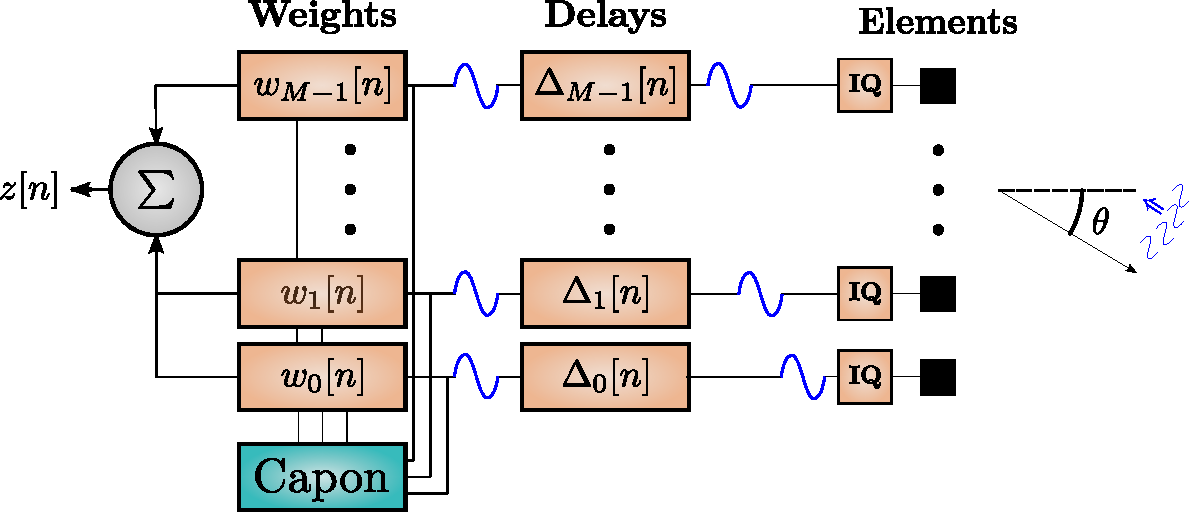
\includegraphics[width=3in]{gfx/beamforming_mv.pdf}}
\caption{Capon beamforming. Impinging signal is demodulated, and aligned in phase by applying steering and focusing delays $\Delta_m[n]$. Adaptive weights, $\vec{w}[n]$, are then calculated based on in-phase data, and finally the output is formed by a Capon-weighted coherent sum.}
\label{fig:mvbf}
\end{figure}

The Capon beamformer can be summerized in three main steps. First a sample covariance matrix has to be calculated, 
\begin{align}
\mat{\breve{R}}[n] = \frac{1}{N_LN_K}\sum_{n'=n-K}^{n+K} \sum_{l=0}^{N_L-1} (\vec{x}_l^{\Delta}[n'])(\vec{x}_l^{\Delta}[n'])^H,\label{eq:R}
\end{align}
where  $N_K = 2K + 1$ is the number of samples included in time, $\vec{x}_l^{\Delta}$ is the $l^\text{th}$ subarray of length $L$ $[x_l^{\Delta}[n], \dotso, x_{l+L-1}^{\Delta}[n]]$ and $N_L = M-L+1$ is the number of subarrays. Note that the covariance matrix dimension is $L \times L$. The covariance matrix is then loaded with a diagonal factor $\epsilon$ to ensure numerical stability and increased robustness, 
\begin{align}\label{eq:diag}
\mat{\hat{R}}[n] =  f(\vec{x}^{\Delta}[n]) = \mat{\breve{R}}[n] + \epsilon[n]\mat{I}.
\end{align}
A weighting proportional to the output power is often used to reduce the need of parameter adjustments, and the trace of $\mat{\breve{R}}$, 
\begin{align}\label{eq:diag_adapt}
\epsilon[n] &= d \times \frac{tr\{\mat{\breve{R}}[n]\}}{L}
\end{align}
has been applied in much of the resent literature on Capon beamforming for medical ultrasound imaging \cite{Synnevag2007, Nilsen2009, Wang2009, Mehdizadeh2012}. This form of adaptive diagonal loading has also been applied to HF and VHF antenna processing \cite{Featherstone1997b}.

Second, a linear system of equations has to be solved
\begin{align}\label{eq:b}
\vec{b}[n] = \mat{\hat{R}}[n]^{-1}\vec{a},
\end{align}
where the steering vector $\vec{a} = \vec{1}_L = [1_0, 1_1, ..., 1_{L-1}]^T$ since $\vec{x}^\Delta$ is pre-delayed. Finally the Capon weight vector is formed based on (\ref{eq:b}) as
\begin{align}\label{eq:w}
\vec{w}[n] = \frac{\vec{b}[n]}{\vec{1}^H\vec{b}[n]},
\end{align}
and the beamformer output is calculated by combining all $N_L$ subarrays weighted with the same set of adaptive weights.
\begin{align}
z[n] &= \frac{1}{N_L}\vec{w}[n]^H \sum_{l=0}^{N_L-1} \vec{x}_l^{\Delta}[n] \label{eq:z_mv}\\
&= 1/N_L \, \text{CONV}_m(\vec{w}[n], \vec{1}_{N_L})^H\vec{x}^{\Delta}[n] \label{eq:z_mv2},
\end{align}
%where (this matrix is wrong)
%\begin{align}
%\mat{C} = \left(
%\begin{matrix}
%\vec{1}_1 & \vec{1}_2 & \cdots & \vec{1}_{N_L} & \vec{0}_1 & \cdots & \vec{0}_{N_L-1} & \vec{0}_{N_L}\\
%\vec{0}_{N_L-1} & \vec{0}_{N_L-2} & \cdots & \vec{0}_{0} & \vec{1}_{N_L-1} & \cdots & \vec{1}_{2} & \vec{1}_{1}\\
%\end{matrix}
%\right)^T
%\end{align}
where $\text{CONV}_m$ is a non-truncated convolution across elements.
Note how we can choose to first sum all subarrays (\ref{eq:z_mv}), or accumulate the right weighting per element (\ref{eq:z_mv2}).

In passive systems, assuming stationary statistics, the sample covariance matrix is typically averaged over a long sequence of samples\cite{Krima}. For an active, pulsed system like medical ultrasound imaging, the available data from which $\mat{\hat{R}}$ can be estimated is quite limited. The resulting sample covariance matrix might therefore be both inaccurate, and poorly conditioned. Another challenge with applying Capon to active systems is the effect of signal cancellation, where high correlation between signal and interference favors weights that cancel out the signal \cite{Reddy1987}. In this way, the beamformer output can be too low at broadside, even when there is signal present and the distortionless-response criterion is applied. 

In order to get a well-conditioned $\mat{\hat{R}}$, avoid signal cancellation, and to get DAS-like speckle, $\mat{\hat{R}}$ has to be averaged over $L\le M/2$ long subarrays and $N_K \sim T_p/T_s$ time samples \cite{Synnevag2007, Synnevag2007a}. Where, $T_p$ is the pulse length in seconds and $T_s$ is the sampling period.

% Få med at vi processerer hele bildet på en gang. Forklar forskjellen med å prosessere en beam av gangen. Hva med MLA?
% Illustrer tråder og tider for hvordan processeringen går.
% Vi snakker om mottak-stråleformeren.

%\begin{figure}
%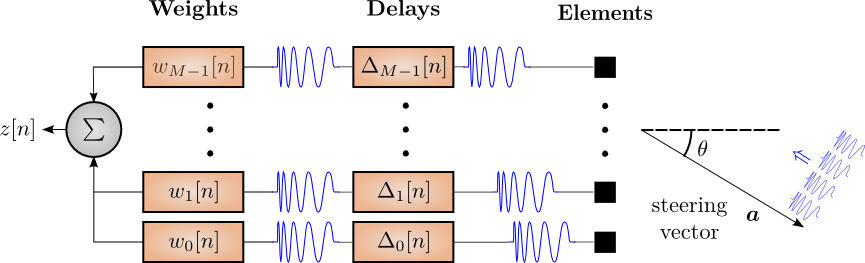
\includegraphics[width=3in]{gfx/beamforming_mv_lowres.png}
%\caption{}
%\label{fig:mv}
%\end{figure}

%Building and calculating the inverse of $\hat{R}$ is computational demanding, limiting the methods accessibility. Following the innovation in GPU computing, this has now started to change. 
%In this paper we introduce the first GPU implementation of the Capon beamformer capable of processing a 70 degree sector cardiac image from a 64 element phased array at interactive frame rates using both spatial and temporal smoothing. Both types of smoothing are important for maintaining delay-and-sum-like speckle and at the same time keep the high resolution property. This is achieved using complex base band data, which reduces the size of each range line to a minimum. In addition, complex data results in complex weights; hence this is a correct implementation of Capon beamforming with all degrees of freedom preserved. For high channel count systems we propose two ways of reducing computational complexity while maintaining 

\subsection{GPU Compute Model}

%\textbf{(Ta med mer banale ting, dette er GPU for ultralydfolk)}

%\textbf{(Etter denne så må de forstå GPU og hvorfor MV passer.)}

In this section we briefly discuss the principle behind GPU computing, laying the basis for further discussion on parallel implementation strategies. CUDA by Nvidia has been our choice of GPU developer environment \cite{Nvidia2011}. However, even though CUDA has been used to implement the Capon beamformer, the challenges and proposed methods described in this paper apply for other massive parallel implementation environments as well, like e.g. OpenCL. The key point is that GPUs can accelerate small concurrent tasks, like beamforming one pixel, much better than a CPU. Where the CPU has few cores and logic to process complex threads, the GPU has many cores, but each thread needs to be simple in order to benefit from the GPU's computational power. 

The CUDA compute model is based on execution of a kernel function across a large set of threads, where the kernel function describe the work to be done in each thread. As depicted in Fig. \ref{fig:gpulayout}, threads are organized in a grid of thread-blocks, with maximal size of 1024 threads per block. Threads inside a block supports low-cost synchronized if needed. From a CUDA perspective the GPU consist of one or more stream multi processors (SMs), where each SM is capable of 32 or more, depending on the architecture, concurrent multiplications and/or additions. A group of blocks is scheduled to each SM until all blocks have been processed. 

A SM has available a limited amount of near-core memory and registers. Each thread therefore has to be as light on memory as possible and has to perform enough instructions per used byte in order to hide memory latency. It is also important that the problem can be divided into enough threads to hide instruction latency. Global reads and writes on the GPU, in addition to CPU-GPU transfers, have high penalty, and should be minimized as much as possible. All of these constraints combined pose a real challenge as the target problem has to map on to the parallel framework both on a grid, block, thread and memory consumption level in order to benefits from parallel acceleration. In the next section, we will describe how this mapping should be done for Capon beamforming of cardiac ultrasound data.    

\begin{figure}
\centerline{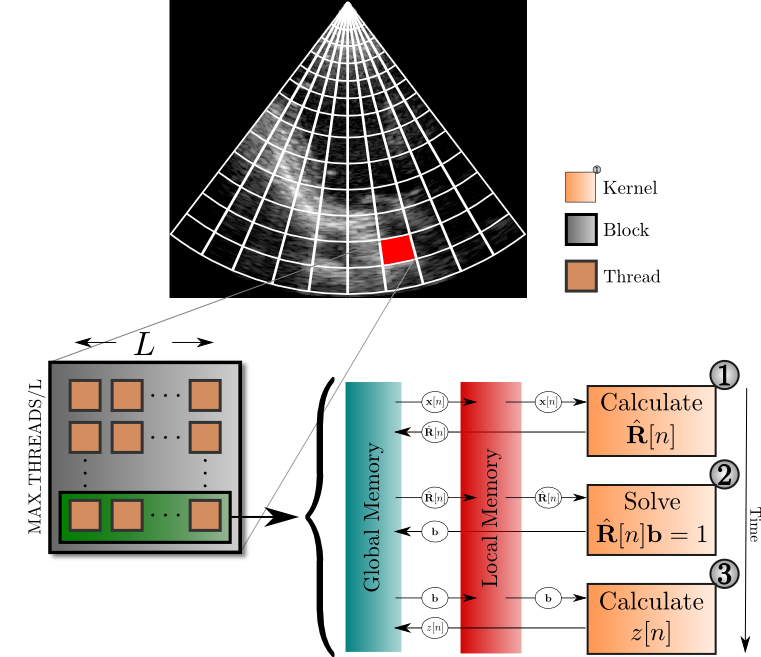
\includegraphics[width=3in]{gfx/gpu_layout_vertical_lr.png}}
\caption{Calculation of Capon adaptive weights mapped to GPU architecture. A recorded echo across the array for a given range and angle (selected cell) is assigned to a group of $L$ threads that can run independently of all other groups. Note that several samples can be processed per block of threads if $L$ is small. The task of these $L$ threads is to calculate the Capon beamformer output in the three depicted steps.}
\label{fig:gpulayout}
\end{figure}

%When implementing algorithms on the GPU it is important to keep data as close to the core as possible. Utilizing available registers and shared memory to its maximum is therefore important.  

%More important, the CUDA 2.x compute capability (CC) has available 48 KB of near-core shared memory per SM that can be utilized by resident blocks. The maximum number of resident blocks per SM is 8, but in addition the maximum number of resident warps per SM is restricted to 48. Hence, with a block size of 512 only $48/(512/32) = 3$ blocks can occupy the SM at once. In addition, if one thread where to use 64B of shared memory the number of allowed resident blocks with a block size of 512 would be reduced to 1. Up to a curtain point it is beneficial to have as many warps as possible occupying the SM at once to hide latency from accessing memory. The SM has for CC 2.x 32K 32-bit long registers. When implementing algorithms on the GPU it is important to keep data as close to the core as possible. Utilizing available registers and shared memory to its maximum is therefore important.  

%\subsection{Optimizing kernel launch}
%Set the size of grid adaptively based on $L$, $M$ and $Yavg$.
%It is better to slide in space than time. $K$ is typically much larger than $2*Yavg + 1$.

% needed in second column of first page if using \IEEEpubid
%\IEEEpubidadjcol

\section{Parallel Capon}\label{sec:meth}
If we analyze the beamformer in (\ref{eq:z_mv}) in combination with (\ref{eq:b}) and (\ref{eq:R}), we see that each calculation of a set of Capon weights is independent across the outputs $z[n]$. As shown in Fig. \ref{fig:gpulayout}, a first level of granularity is therefore to divide the image into a grid, where the output in each cell can be calculated independently of all others. Further, based on memory dependencies and to hold memory consumption per thread at a minimum, one should recognise that a group of threads should process one output in the final image. Continuing with the calculation of one weight vector, the algorithm can be broken down into three main steps that, to some extent, can be further divided into a small set of parallel processes. That is, for each data vector $\vec{x}^\Delta$ in the image:
\begin{align*}
%\begin{array}{l}
\text{1) } &\text{Calculate the sample covariance matrix } \mat{\hat{R}} \text{ as in } \text{(\ref{eq:diag})}\\
\text{2) } &\text{Solve the linear system of equations in (\ref{eq:b}})\\ %\vec{b} =\mat{\hat{R}}^{-1}\vec{1}_L\\
\text{3) } &\text{Calculate } \vec{w} = \vec{b}/\vec{1}_{L}^H\vec{b} \text{ and the amplitude as in (\ref{eq:z_mv})}
%\end{array}
\end{align*}
%\begin{enumerate}
%\item Calculate the sample covariance matrix $\mat{\hat{R}}$ as in (\ref{eq:R})
%\end{enumerate}
%\begin{enumerate}
%\item[2)] Solve the linear system of equations $\mat{\hat{R}}\vec{b} =\vec{ 1}$
%\end{enumerate}
%\begin{enumerate}
%\item[3)] Calculate $\vec{w} = \vec{b}/\vec{1}^H\vec{b}$ and the amplitude $\vec{w}^H\vec{x}$
%\end{enumerate}
The computational complexity of these three steps is $O(L^3)$, $O(L^3)$, and $O(L)$ respectively. As $L$ increases, the first two steps quickly become unmanageable, and real-time performance can only be achieved by exploring novel solutions to reduce complexity. 

%(The three steps have, for modularity, been implemented using three different kernels. Joining all kernels into one could possible lead to an increase in speed.)

%\begin{figure}
%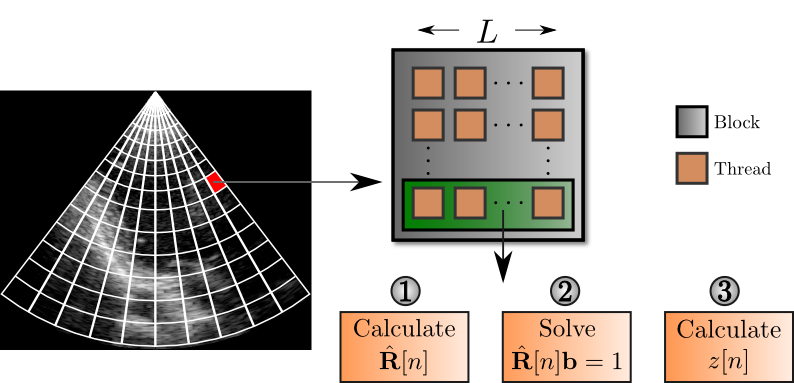
\includegraphics[width=3in]{gfx/gpu_layout_lowres.png}%
%\caption{}
%\label{fig:gpulayout}
%\end{figure}

\subsection{Calculating Multiple Sample Covariance Matrices}\label{sec:calcR}

%The straightforward sum in (\ref{eq:R}) has complexity $O(L^2N_LN_K) = O(L^3)$ since $N_L$, the number of subarrays, is a function of $L$. This is actually the same as for inverting an $L \times L$ matrix. However little attention has been devoted to this step in the literature before. Note that for a typical array configuration we do more spacial smoothing than temporal smoothing. Hence, $N_K$ is usually small compared to $N_L$. The construction of $\mat{\hat{R}}$ is dominated by the number of elements $M$ ($N_L = M - L + 1$) for short subarrays, but since $L$ is selected in most cases to be between $M/2$ and $M/4$ a large $M$ implies a large $L$.

From (\ref{eq:R}) it is obvious that calculation of one element in $\mat{\hat{R}}$ is independent of all the other elements. A natural level of granularity would then be to assign one thread to each element of $\mat{\hat{R}}$ as in \cite{Chen2011}. This will minimize global reads and writes needed per thread, but unfortunately the maximum number of threads per block puts an upper limit on the subarray length, $L_{max}=32$, since we want to avoid block-to-block synchronization.

The cubic complexity with $L$ and linear complexity with $N_K$ can be reduced by realizing that the calculation in (\ref{eq:R}) overlap both across subarrays and in time. Element $(i,j)$ of $\mat{\breve{R}}[n]$ can be calculated from element $(i-1, j-1), \text{for } i,j \in [1, L-1]$ as
\begin{align}
\mat{\breve{R}}_{i,j}[n] &=  \mat{\breve{R}}_{i-1,j-1}[n]  \nonumber \\
&+ \sum_{n'=n-K}^{n+K} (x_{i+N_L-1}^{\Delta}[n']x_{j+N_L-1}^{\Delta}[n']^* \nonumber \\
&- x_{i-1}^{\Delta}[n']x_{j-1}^{\Delta}[n']^H) \label{eq:sliding}
\end{align}
The same is true in time where
\begin{align}
\mat{\breve{R}}[n] &= \mat{\breve{R}}[n-1] + \sum_{l=0}^{N_L-1} (\vec{x}^{\Delta}_l[n+K]\vec{x}^{\Delta}_l[n+K]^H \nonumber \\
&- \vec{x}^{\Delta}[n-K-1]\vec{x}^{\Delta}[n-K-1]^H).
\end{align}
%- \mat{\breve{R}}[n-K-1] + \mat{\breve{R}}[n-K].
Both sliding across subarrays and in time can be realized simultaneously if we hold a $N_K$-average in time of the outer products $\vec{x}^{\Delta}[n]\vec{x}^{\Delta}[n]^H$ in memory and calculate $\mat{\hat{R}}$ averaged over subarrays from this buffer (cite JOE?). However, since $N_K$ typically is small, and we have a limited amount of memory available per thread, we have chosen to focus on sliding across subarrays only (\ref{eq:sliding}). In that case, the complexity of calculating $\mat{\hat{R}}$ is reduced to $O(L^2)$. Notice how sliding will break independence along the sliding dimension. With our choice of calculating $\mat{\hat{R}}$, calculations are still independent across time, but not along diagonals in $\mat{\hat{R}}$. We therefore have selected to use one thread per diagonal in the upper triangle of $\mat{\hat{R}}$, and for small values of $L$, several covariance matrices are calculated per thread block (Fig. \ref{fig:gpulayout}). Maximum supported $L$ is with this approach increased to 512, however for small $L$ high $M$ configurations, memory consumption per thread will be to high to achieve full occupancy of the GPU.

Taking symmetry into account, only the upper half of $\mat{\hat{R}}$ needs to be calculated. However, the way we have decided to organize the GPU compute threads per $\mat{\hat{R}}$, the lower triangle can be calculated with little overhead on the GPU. This also means that we do not rely on a symmetric solver to solve $\mat{\hat{R}}\vec{b} = \vec{1}_L$, even if that could have saved some instructions.

Diagonal loading as a constant value can be added with marginal cost. For the adaptive diagonal loading factor in (\ref{eq:diag}), the trace of $\mat{\hat{R}}$ has to be known before diagonal elements are written back to global memory. Since one row for all covariance matrices is written to global memory per kernel iteration, the diagonal elements need to be held in a local memory until the trace is accumulated. When it is found, scattered writes of the diagonal elements to global memory has to be performed. 

%For subarray averaging, the first row and column of $\mat{\hat{R}}$ has to be fully calculated, and for time averaging $\mat{\hat{R}}[0]$ has to be fully calculated.

%Since $L$ usually is larger than $N$, we have 

%Building $\hat{\mat{R}}$ using a sliding window approach across $K$ and $N_{avg}$. We have a limited amount of fast, near-core memory on the GPU. On NVIDIA architecture this memory is known as shared memory, and is restricted to 48KB per compute block. The maximum block size of 32x32, further restrict how large arrays we can handle inside a single compute block. It is therefore natural to restrict $L$ to a maxima of $32$ elements. Since $L \le M/2$, $M \le 64$. We can not afford to hold the full $\hat{\mat{R}}$ ($M = L$) when $\hat{\mat{R}} > 32$, because of limited amount of memory. ... Explain in detail how \texttt{buildR} is implemented in a kernel. ... Give more details on how much shared memory we have, and how it can be divided between compute blocks occupying one stream multiprocessor (SM).

%Discuss the bottleneck adaptive diagonal loading causes. Possible solutions includes, use trace from previous image, use pre-calculated array power, constant weight.

%Time averaging takes a lot of resources. It has been shown that time averaging can maintain both resolution and delay-and-sum-like speckle. The same speckle statistics can be obtain with small subarrays, but then we loose resolution. Small sub-arrays benefits from being less computational demanding.   

%\subsubsection{CUDA Compute Model}
%The CUDA compute model is based on execution of a kernel across a grid of compute threads. Each position in the grid holds a block of threads. Each block is further divided into groups of 32 threads, known as a warp. The maximum number of threads inside a block is restricted to 512, hence 16 warps. From a CUDA perspective the GPU consist of one or more stream multi processors (SM), %where each SM is capable of 32 or more, depending on the architecture, concurrent multiplications and/or additions. The CUDA 2.x compute capability (CC) has available 48 KB of near-core shared memory per SM that can be utilized by resident blocks. The maximum number of resident blocks per SM is 8, but in addition the maximum number of resident warps per SM is restricted to 48. Hence, %with a block size of 512 only $48/(512/32) = 3$ blocks can occupy the SM at once. In addition, if one thread where to use 64B of shared memory the number of allowed resident blocks with a block size of 512 would be reduced to 1. Up to a curtain point 
%it is beneficial to have as many warps as possible occupying the SM at once to hide latency from accessing memory and executing time consuming mathematical functions. The SM has for CC 2.x 32K 32-bit long registers. When implementing algorithms on the GPU it is important to keep data as close to the core as possible. Utilizing available registers and shared memory to its maximum is %therefore important.   

\subsection{Solving Multiple Small Linear Systems}
In the literature, when it comes to solving systems of linear equations on the GPU the focus has mostly been on large systems, and GPU libraries therefore often lack a comprehensive collection of batched solvers. The reason for this is two-fold, first the GPU needs to solve thousands of small systems in order to beat the low memory latency of the CPU, second there is a range of system dimensions that does not fit well with the GPU architecture, where only a small amount of near-core memory and registers are available. Because of this, it has been proven hard to optimize a manageable set of solvers that provides speedups compared with the CPU in every cases. It is therefore not given that solving on the GPU is faster than solving on the CPU in general. However, there is two arguments for doing solving on the GPU. First the CPU, which might already runs a lot of algorithms, is offloaded. Second the transfer of several thousand covariance matrices from CPU-side to GPU-side is spared.

For the results presented in this paper, we have used an unreleased GPU implementation of Gauss-Jordan (GJ) elimination (by Nvidia) to solve $\mat{\hat{R}}\vec{b} = \vec{1}_L$, where $\vec{b} = \mat{\hat{R}}^{-1}\vec{1}_L$. %For smaller systems, $L < 10$, a direct solver using one thread per system is preferable. For this purpose we have implemented Cramer's rule for $2 \times 2$, $3 \times 3$ and $4 \times 4$ matrices. All solvers have been benchmarked against the latest Intel MKL libraries.

%However we will go through an implementation of an $\mat{U}^H\mat{D}\mat{U}$-decomposition-based solver to point out challenges when implementing batched solving of small linear systems on the GPU. ... (Unsure if this should be included).

%Can include details on GPU implementation of $\mat{U}^H\mat{D}\mat{U}$, but this has not proved to be faster than NVIDIA's GJ implementation. However, the complexity for solving with $\mat{U}^H\mat{D}\mat{U}$ decomposition is supposed to be $1/2$ of GJ.

%Skriv om utfordringene om å lage en solver på GPU. Ikke dra inn UHDU.

%In the final journal article we could discuss Conjugated gradient and Woodbury and the benefits they bring.
%Other solvers that provides different benefits includes Conjugated gradient and the use of the Woodbury matrix identity. 

\subsection{Compute Beamformer Output}
To calculate the beamformer output we have implement the formula in (\ref{eq:z_mv}) with one thread per element-weight ($L$ threads per weight vector). After the solution vector $\vec{b}$ has been placed in shared memory, one of the $L$ threads finds the sum of $\vec{b}$. Another option is to let several threads cooperate to form the sum using a binary reduction sum. However, in the following benchmarks the first approach has been used. Each of the $L$ threads then read one element of $\vec{b}$, scale it with the inverse sum just found to get the weight vector $\vec{w}[n]$. 

The final output, as shown in (\ref{eq:z_mv}) and (\ref{eq:z_mv2}), can be formed by either reducing the data down to length $L$, or increase the weight vector to length $M$. Since we have decided to have $L$ threads per output, the data is reduced to length $L$ by letting thread $r$ calculate 
\begin{align}\label{eq:subsum}
\breve{x}_{r}^{\Delta} = \sum_{k=r}^{r+N_L-1}x_{k}^{\Delta} \text{ for } r \in [0, L-1].
\end{align}
Each thread now computes $z_r = w_r^*x_r$, and finally one thread computes and outputs $z = \frac{1}{N_L}\sum_{r=0}^{L-1} z_r$ to global memory. The last sum can also be performed using a binary reduction sum across several threads for increased speed.

\section{Beamspace Processing}\label{sec:bs}
Nilsen et al. \cite{Nilsen2009} have proposed to apply beamspace processing to further reduce the required computations for the Capon beamformer. With beamspace we mean transforming the channel data from element space to a fan of beams covering the sector illuminated by transmit beams. The transformation is written as
\begin{align}
\vec{x}_{BS}[n] &= \mat{B}\vec{x}^{\Delta}[n], \ \ \ \mat{B} \in C^{M,M}\\
[\mat{B}]_{p,q} &= \frac{1}{\sqrt{M}}e^{-j 2 \pi p q / M}.
\end{align} 
The steering vectors in $\mat{B}$, the so-called Butler matrix, determine each beam's direction in space. We can therefore easily remove beams where no interference is present by removing rows from $\mat{B}$. 

For a focused system like cardiac ultrasound imaging, where the received signal is concentrated in a narrow band around broadside, there is a small percentage of the beams that contains almost all the energy. Nilsen et al. concluded that as little as three beams around broadside were adequate to produce results comparable to applying Capon beamforming in element space. Hence, the inversion steps is found to be constant with respect to the number of array elements.

The beamspace version of the Capon beamformer is derived by replacing the covariance matrix in (\ref{eq:w}) with the beamspace covariance matrix $\mat{\hat{R}}_{BS} = f(\vec{x}_{BS}) = f(\mat{B}\vec{x})$, where $\mat{B} \in \mathbb{C}^{N_b,L}$, and $N_b$ is the number of selected beams. The transformation must be done per subarray, yielding subarrays that no longer overlap in space. If the transformation is applied before the covariance matrix is constructing, the amount of input data is change from $M$ to $N_LN_b$ elements per sample, however all remaining steps will get lower complexity.

Another choice is to transform the element space covariance matrix to beamspace. 
\begin{align}
\mat{\hat{R}}_{BS} &= \mat{B}\mat{\hat{R}}\mat{B}^H
\end{align}
The pros using this approach is that minor changes has to be made to the pipeline described in Section \ref{sec:meth}, but it will only speed up the solving step if the solution $\vec{b}_{BS}$ is transformed back to element space. In this paper we will describe how the first approach has been implemented on the GPU.
%By this approach we go from solving $\mat{\hat{R}}\vec{b} = \vec{1}_L$, which is an $L \times L$ system, to solving the $N_b \times N_b$ system $\mat{\hat{R}}_{BS}\vec{b}_{BS} = (\sqrt{L}\vec{e}_1)$. Now, one can either choose to transform the subarray sums, as in (\ref{eq:subsum}), to beamspace or transform the result, $\vec{b}_{BS}$, back to element space. 
In both cases solving has to be performed against a transformed steering vector
\begin{align}
\vec{a}_{BS} &= \mat{B}\vec{1}_L = \sqrt{L}\vec{e}_1,
\end{align}
where $\vec{e}_i$ has value one in the i$^{th}$ position and is zero elsewhere.

%The implementation calculating covariance matrices therefore needs to be adjusted to handle non-overlapping subarrays. The complexity of constructing the covariance matrix is changed to $O(N_b^2L)$, so constructing the covariance matrices will be faster in beamspace as long as $N_b < \sqrt{L}$.
%Derivation of sliding beamspace transformation. 
Given a $M$ long data vector divided into $N_L$ subarrays, the beamspace transformation of the $l^{th}$ subarray is given as:
\begin{align}\label{eq:bs_formula}
x_{BS,l,k} = \frac{1}{\sqrt{L}}\sum_{p=i}^{l+L-1}x_p e^{-j2\pi k(p-l)/L} , k \in [0, N_b-1].
\end{align}
Manipulating this expression we find that for $l \in [1, L-1]$
\begin{align}\label{eq:sliding_bs}
x_{BS,l,k} &= \frac{1}{\sqrt{L}}((x_{BS,l-1,k} - x_{l-1})e^{-j2\pi k/L} \nonumber \\ &+ x_{i+L-1}e^{-j2\pi k(L-1)/L}) \nonumber \\
&= \frac{1}{\sqrt{L}}(x_{BS,l-1,k} - x_{l-1} + x_{i+L-1})e^{-j2\pi k/L}.
\end{align}
We call this the sliding beamspace transformation (SBS), and it is equal to a normalized sliding DFT. For $l=0$ a full computation has to be performed using (\ref{eq:bs_formula}).

From (\ref{eq:sliding_bs}) it is obvious that instructions can be saved if we utilize the overlap across subarrays, with an increase in task parallel granularity (As discussed in Section \ref{sec:calcR}). With SBS we can therefore select to have one thread per beam (index $k$) that calculates this beam for all subarrays. However, since the number of beams usually is small we will end up with a large memory per thread ratio ($M \gg N_b$). Using one thread per beam is therefore not feasible for small $N_b$ large $M$ configurations. The solution is to combine SBS with full computations. As shown in Fig. (???), a number of thread groups target different sets of subarrays which they transform using the SBS algorithm. In that way, the number of threads per sample is increased and thus the memory per thread ratio is decreased. 

As mentioned the amount of data is increased from $M$ to $N_LN_b$ per sample in beamspace. This means that we no longer can exploit spatial overlap when calculating the sample covariance matrix, but since $N_b$ is small we can now allow to have one thread per element in $\mat{\hat{R}}_{BS}$. A kernel similar to the one described by Chen et al. \cite{Chen2011}, has therefore been implemented. For small $N_b$ values, several covariance matrices are calculated per thread block to achieve high occupancy of the SMs.

After solving $\vec{b}_{BS} = \sqrt{L}\mat{\hat{R}}_{BS}^{-1}\vec{e}_1$, the beamspace weight vector is calculated as 
\begin{align}
\vec{w}_{BS} = \frac{\vec{b}_{BS}}{\sqrt{L}\vec{e}_1\vec{b}_{BS}}
\end{align}  
and applied to the beamspace data summed across subarrays.

%How do we calculate the number of possible subarrays $N_L$ with overlap $L-s$ in a data vector of length $M$.
%\begin{align}
%N_L = floor(\frac{M}{s}) - floor(\frac{L-1}{s})
%\end{align}

As presented in (\ref{eq:diag}), adaptive diagonal loading is performed by loading the sample covariance matrix with the average energy per element, hence $trace\{\mat{\hat{R}}\}/L$. If adaptive diagonal loading is applied after data has been transformed into beamspace, a high percentage of the total energy is mapped to a small subset of beams. Thus the average energy per beam is higher than the average energy per element, if the system uses focused transmit beams. This means that less diagonal loading has to be applied in beamspace than in element space ($d_{BS} \ll d_{element}$).

%(Go in detail about the implementation using sliding DFT).

%(Go in detail about what kind of modifications we need to do to each of the three steps)

%Note that $\mat{B}\mat{B}^H = \mat{I}$ and $\mat{B}^H\mat{B} \ne \mat{I}$ when $N_b < L$.

%Another way of computing the beamspace transformation is to transform the steering vector $\vec{a}$ and covariance vector $\mat{\hat{R}}$ beforing solving the following system of linear equations: $(\mat{B}\mat{\hat{R}}\mat{B}^H)^{-1}(\mat{B}a) = b_{BS}$.

%\subsection{Iterative Capon}
%The idea behind iterative Capon is to perform Capon using small subarrays in several iterations until there is only two subarrays to sum. In this way we fix the size of L, hence the complexity of solving $\mat{R}\vec{b} = \vec{1}$. However, for each iteration we re-obtain L-1 degrees of freedom until all are retrieved after $K = M-L+1$ iterations. Since subarray averaging has been applied to decorrelated the signal, we might loose this effect when reestablishing all degrees of freedom. The number of iterations should therefore be restricted to $K/2$ to equal the normal choice of $L = M/2$ when it comes to degrees of freedom. 
 

\section{Results}\label{sec:res}
Describe the computer system (CPU, GPU...). Describe the data that are processed (field II, Channel data from GE Vingmed).
% stolpediagram, med de ulike metodenes kjøretid oppehverandre.

\begin{figure*}[!t]
\centerline{\subfloat[]{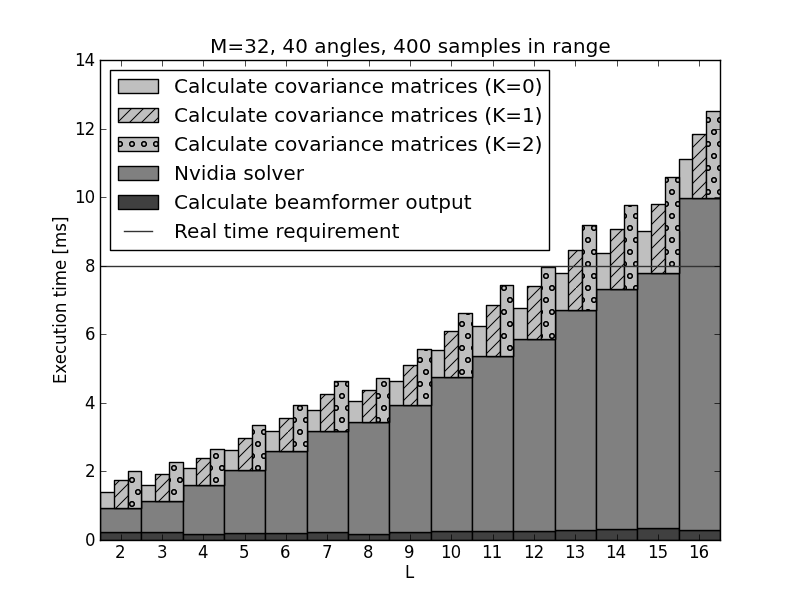
\includegraphics[width=3.5in]{gfx/benchmark_bar_32_40_400.png} \label{fig:benchUS32}}
\hfil
\subfloat[]{\includegraphics[width=3.5in]{gfx/benchmark_bar_64_80_400.png}%
\label{fig:benchUS64}}}
\caption{(Change into bar plot?) Benchmark of GPU Capon beamforming for a cardiac image covering a 70 degrees sector. Execution time is plotted as a function of subarray length $L$. The plot shows execution times for the three steps listed in Section \ref{sec:meth}. Calculating covariance matrices in red, solver in green, and the final beamformer sum in blue. For each step, there is one line for three different choices of temporal averaging, $N_{avg} \in [0, 1, 2]$. (a) A 32 element array. (b) A 64 element array.}
\label{fig:bench}
\end{figure*}

\begin{figure*}[!t]
\centerline{\subfloat[]{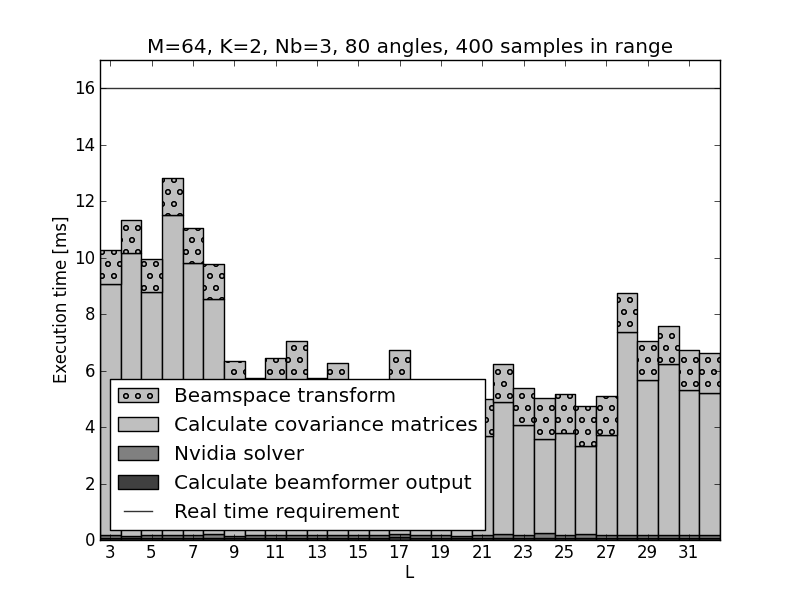
\includegraphics[width=3.5in]{gfx/benchmark_bar_bs_M=64_Nx=80_Ny=400_Nb=3.png} \label{fig:benchBS3}}
\hfil
\subfloat[]{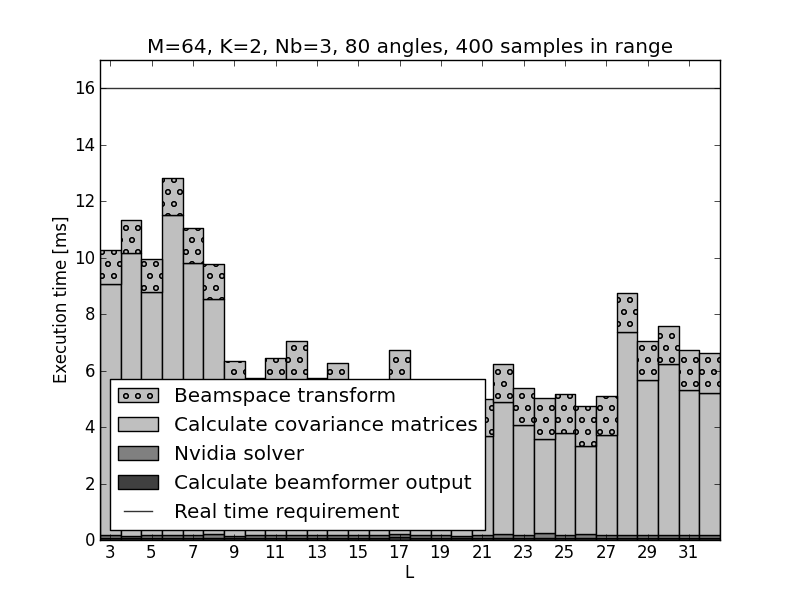
\includegraphics[width=3.5in]{gfx/benchmark_bar_bs_M=64_Nx=80_Ny=400_Nb=3.png}%
\label{fig:benchBS5}}}
\caption{(TODO: Add the right figure. Change it into a bar plot?) Benchmark of GPU Beamspace Capon beamforming for a cardiac image covering a 70 degrees sector. Execution time is plotted as a function of number of elements $M$. The plot shows execution times for the three steps listed in Section \ref{sec:meth}. Calculating covariance matrices in red, solver in green, and the final beamformer sum in blue. For each step, there is one line for three different choices of temporal averaging, $N_{avg} \in [0, 1, 2]$. (a) 3 beams. (b) 5 beams.}
\label{fig:benchBS}
\end{figure*}

\begin{figure*}[!t]
\centerline{\subfloat[]{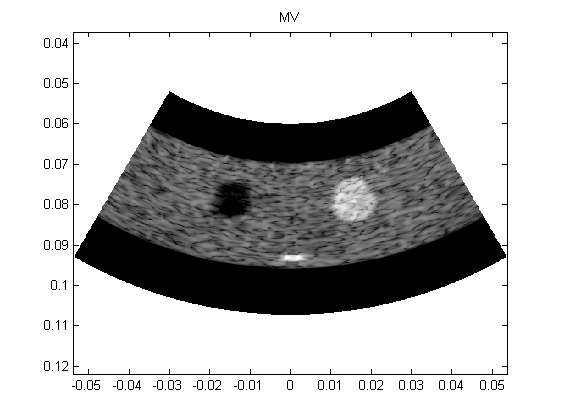
\includegraphics[width=2in]{gfx/mv_phantom.png} \label{fig:phantomDAS}}
\hfil
\subfloat[]{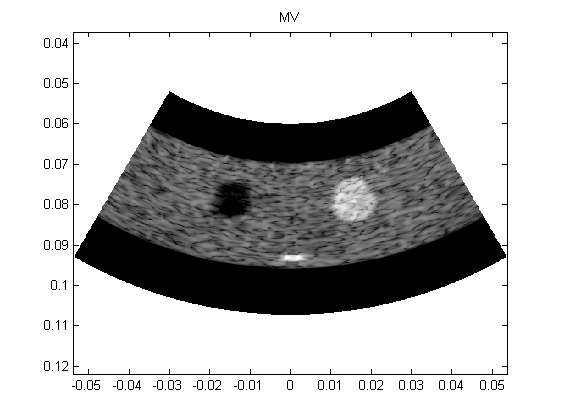
\includegraphics[width=2in]{gfx/mv_phantom.png} \label{fig:phantomMV}}
\hfil
\subfloat[]{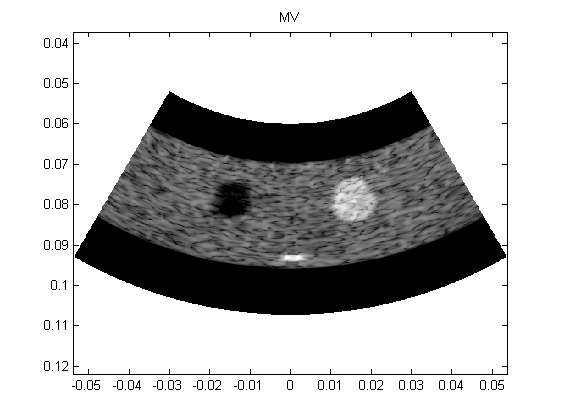
\includegraphics[width=2in]{gfx/mv_phantom.png} \label{fig:phantomBS}}}
\caption{(TODO: Add the right figures) Have graph showing cyst contrast as a function of different parameters instead? Cyst and point targets phantom a) Delay-and-sum, uniform weights. b) Capon ($M=?, L=?, N=?$) c) Beamspace Capon ($M=?, L=?, N=?, N_b=?$).}
\label{fig:bench}
\end{figure*}

\begin{figure*}[!t]
\centerline{\subfloat[]{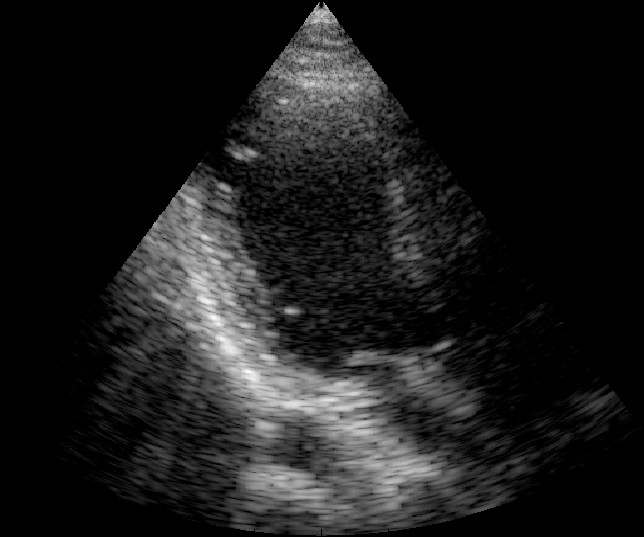
\includegraphics[width=2in]{gfx/us_image.png} \label{fig:phantomDAS}}
\hfil
\subfloat[]{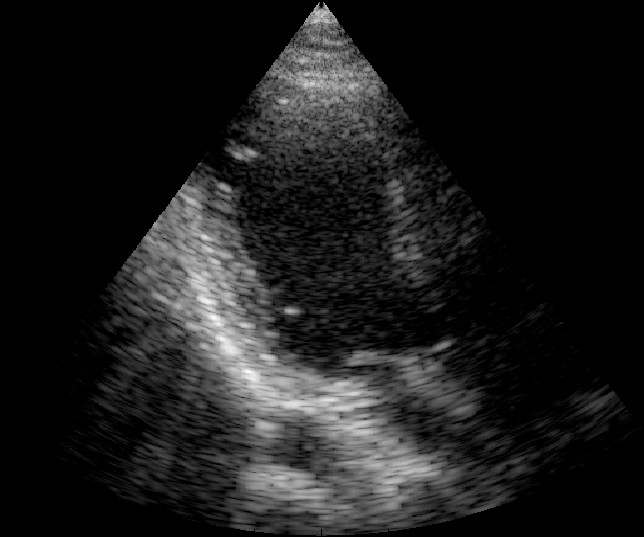
\includegraphics[width=2in]{gfx/us_image.png} \label{fig:phantomMV}}
\hfil
\subfloat[]{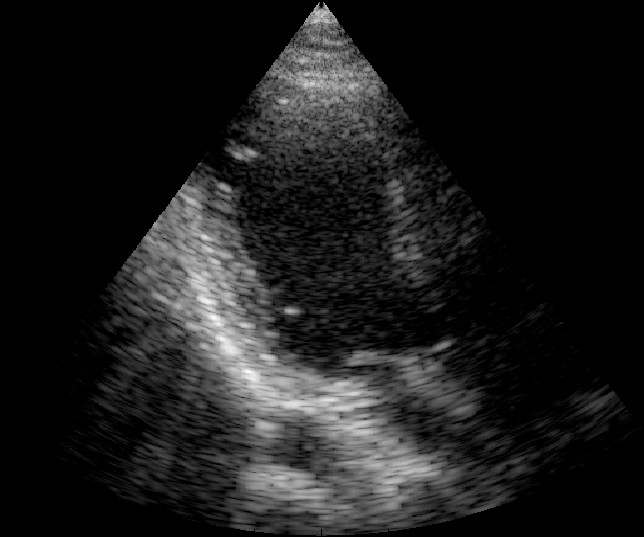
\includegraphics[width=2in]{gfx/us_image.png} \label{fig:phantomBS}}}
\caption{(TODO: Add the right figures) Have graph showing cavity-wall contrast as a function of parameters instead? In-vivo cardiac ultrasound image a) Delay-and-sum, uniform weights. b) Capon ($M=?, L=?, N=?$) c) Beamspace Capon ($M=?, L=?, N=?, N_b=?$).}
\label{fig:bench}
\end{figure*}

Present images before and after Capon weights has been applied. Comment on the effect of selecting different parameters. Present graph showing executing times for Cython-Capon v.s. CUDA-Capon for different choices of parameters. Comment on different choices of parameters change the running times. Temporal averaging for instance, lowers the efficiency since $2Y_{avg}$ more operations has to be performed per $\mat{\hat{R}}$    

Present images, both simulated and in-vivo, processed using beamspace Capon. Comment on the differences between the two and on how much they deviates from the full method.
%Show beampatterns for the two compared with the full method. 
Show executing times for the two methods compared with the full method on the GPU.

Describe the base band (IQ-demodulation) process that the data has been undergoing.

How has the data been acquired?

Ta med en serie med bilde. Må vise tydelig at det gir forbedring. 

Add a comparison between beamspace and full capon using small L.

\section{Discussion}\label{sec:dis}
Discuss results presented in Section \ref{sec:res}.

We expect that a large speedup had the Capon beamformer been implemented on the CPU using threads and SIMD (single instruction multiple data) instructions. 

Solving linear systems on the GPU is not believed to be much faster than a CPU implementation, but there is two key points. First the CPU is offloaded, and second the time it takes to transfer all covariance matrices back to the CPU makes the choice of doing the solving on the GPU simple to make.

(results)?
For a typical cardiac ultrasound image of 80*400 pixels (70 degree sector, 15cm range) acquired using a 2.5MHz, $M=64$ element phased array, the result is 10fps (subarray length $L=M/2$, temporal smoothing over 3 samples). If we do a 2-element pre-beamforming to get the channel count down to 32, the frame rate increases to 44fps. For a 32 element phased array we need less beams to cover the sector ($40 \times 400$ pixels), hence with the same parameters the frame rate increases to 87fps. The bottleneck of the Capon algorithm is to find the inverse covariance matrix for all pixels. This is an $O(L^3)$ operation, and results show that when L is larger than 16, real time performance is not possible for cardiac imaging with current high-end hardware. The target GPU has been Nvidia’s Quadro 6000, capable of 1Tflops.

Toeplitz-based solver (cite new article). Discuss it.

How does beamspace perform when using plane wave imaging...?

\section{Conclusion}\label{sec:con}
...


% An example of a floating figure using the graphicx package.
% Note that \label must occur AFTER (or within) \caption.
% For figures, \caption should occur after the \includegraphics.
% Note that IEEEtran v1.7 and later has special internal code that
% is designed to preserve the operation of \label within \caption
% even when the captionsoff option is in effect. However, because
% of issues like this, it may be the safest practice to put all your
% \label just after \caption rather than within \caption{}.
%
% Reminder: the "draftcls" or "draftclsnofoot", not "draft", class
% option should be used if it is desired that the figures are to be
% displayed while in draft mode.
%
%\begin{figure}[!t]
%\centering
%\includegraphics[width=2.5in]{myfigure}
% where an .eps filename suffix will be assumed under latex, 
% and a .pdf suffix will be assumed for pdflatex; or what has been declared
% via \DeclareGraphicsExtensions.
%\caption{Simulation Results}
%\label{fig_sim}
%\end{figure}

% Note that IEEE typically puts floats only at the top, even when this
% results in a large percentage of a column being occupied by floats.


% An example of a double column floating figure using two subfigures.
% (The subfig.sty package must be loaded for this to work.)
% The subfigure \label commands are set within each subfloat command, the
% \label for the overall figure must come after \caption.
% \hfil must be used as a separator to get equal spacing.
% The subfigure.sty package works much the same way, except \subfigure is
% used instead of \subfloat.
%
%\begin{figure*}[!t]
%\centerline{\subfloat[Case I]\includegraphics[width=2.5in]{subfigcase1}%
%\label{fig_first_case}}
%\hfil
%\subfloat[Case II]{\includegraphics[width=2.5in]{subfigcase2}%
%\label{fig_second_case}}}
%\caption{Simulation results}
%\label{fig_sim}
%\end{figure*}
%
% Note that often IEEE papers with subfigures do not employ subfigure
% captions (using the optional argument to \subfloat), but instead will
% reference/describe all of them (a), (b), etc., within the main caption.


% An example of a floating table. Note that, for IEEE style tables, the 
% \caption command should come BEFORE the table. Table text will default to
% \footnotesize as IEEE normally uses this smaller font for tables.
% The \label must come after \caption as always.
%
%\begin{table}[!t]
%% increase table row spacing, adjust to taste
%\renewcommand{\arraystretch}{1.3}
% if using array.sty, it might be a good idea to tweak the value of
% \extrarowheight as needed to properly center the text within the cells
%\caption{An Example of a Table}
%\label{table_example}
%\centering
%% Some packages, such as MDW tools, offer better commands for making tables
%% than the plain LaTeX2e tabular which is used here.
%\begin{tabular}{|c||c|}
%\hline
%One & Two\\
%\hline
%Three & Four\\
%\hline
%\end{tabular}
%\end{table}


% Note that IEEE does not put floats in the very first column - or typically
% anywhere on the first page for that matter. Also, in-text middle ("here")
% positioning is not used. Most IEEE journals use top floats exclusively.
% Note that, LaTeX2e, unlike IEEE journals, places footnotes above bottom
% floats. This can be corrected via the \fnbelowfloat command of the
% stfloats package.



%\section{Conclusion}
%The conclusion goes here.





% if have a single appendix:
%\appendix[Proof of the Zonklar Equations]
% or
%\appendix  % for no appendix heading
% do not use \section anymore after \appendix, only \section*
% is possibly needed

% use appendices with more than one appendix
% then use \section to start each appendix
% you must declare a \section before using any
% \subsection or using \label (\appendices by itself
% starts a section numbered zero.)
%


%\appendices
%\section{Proof of the First Zonklar Equation}
%Appendix one text goes here.

% you can choose not to have a title for an appendix
% if you want by leaving the argument blank
%\section{}
%Appendix two text goes here.


% use section* for acknowledgement
\section*{Acknowledgment}


The authors would like to thank...


% Can use something like this to put references on a page
% by themselves when using endfloat and the captionsoff option.
\ifCLASSOPTIONcaptionsoff
  \newpage
\fi



% trigger a \newpage just before the given reference
% number - used to balance the columns on the last page
% adjust value as needed - may need to be readjusted if
% the document is modified later
%\IEEEtriggeratref{8}
% The "triggered" command can be changed if desired:
%\IEEEtriggercmd{\enlargethispage{-5in}}

% references section

% can use a bibliography generated by BibTeX as a .bbl file
% BibTeX documentation can be easily obtained at:
% http://www.ctan.org/tex-archive/biblio/bibtex/contrib/doc/
% The IEEEtran BibTeX style support page is at:
% http://www.michaelshell.org/tex/ieeetran/bibtex/
\bibliographystyle{IEEEtran}
% argument is your BibTeX string definitions and bibliography database(s)
%\bibliography{IEEEabrv,../bib/paper}
\bibliography{mybib} % link to mendeley organized bibtex-file
%\bibliography{IEEEabrv,mybib} 
% <OR> manually copy in the resultant .bbl file
% set second argument of \begin to the number of references
% (used to reserve space for the reference number labels box)
%\begin{thebibliography}{1}

%\bibitem{IEEEhowto:kopka}
%H.~Kopka and P.~W. Daly, \emph{A Guide to \LaTeX}, 3rd~ed.\hskip 1em plus
%  0.5em minus 0.4em\relax Harlow, England: Addison-Wesley, 1999.

%\end{thebibliography}

% biography section
% 
% If you have an EPS/PDF photo (graphicx package needed) extra braces are
% needed around the contents of the optional argument to biography to prevent
% the LaTeX parser from getting confused when it sees the complicated
% \includegraphics command within an optional argument. (You could create
% your own custom macro containing the \includegraphics command to make things
% simpler here.)
%\begin{biography}[{\includegraphics[width=1in,height=1.25in,clip,keepaspectratio]{mshell}}]{Michael Shell}
% or if you just want to reserve a space for a photo:

% insert where needed to balance the two columns on the last page with
% biographies
%\newpage

\begin{IEEEbiography}{Jon Petter \AA{}sen}
Biography text here.
\end{IEEEbiography}

\begin{IEEEbiography}{Jo Inge Buskenes}
Biography text here.
\end{IEEEbiography}

\begin{IEEEbiography}{Carl-Inge Colombo Nilsen}
Biography text here.
\end{IEEEbiography}

% insert where needed to balance the two columns on the last page with
% biographies
%\newpage

\begin{IEEEbiography}{Andreas Austeng}
Biography text here.
\end{IEEEbiography}

\begin{IEEEbiography}{Sverre Holm}
Biography text here.
\end{IEEEbiography}


% You can push biographies down or up by placing
% a \vfill before or after them. The appropriate
% use of \vfill depends on what kind of text is
% on the last page and whether or not the columns
% are being equalized.

%\vfill

% Can be used to pull up biographies so that the bottom of the last one
% is flush with the other column.
%\enlargethispage{-5in}



% that's all folks
\end{document}


